%%%%%%%%%%%%%%%%%%%%%%%%%%%%%%%%%%%%%%%%%
% Beamer Presentation
% LaTeX Template
% Version 1.0 (10/11/12)
%
% This template has been downloaded from:
% http://www.LaTeXTemplates.com
%
% License:
% CC BY-NC-SA 3.0 (http://creativecommons.org/licenses/by-nc-sa/3.0/)
%
%%%%%%%%%%%%%%%%%%%%%%%%%%%%%%%%%%%%%%%%%

%-------------------------------------------------------------------------------
%	PACKAGES AND THEMES
%-------------------------------------------------------------------------------

%\documentclass{beamer}
\documentclass[12pt, aspectratio=169]{beamer}
\usepackage{keynote-gradient}

\mode<presentation> {

% The Beamer class comes with a number of default slide themes
% which change the colors and layouts of slides. Below this is a list
% of all the themes, uncomment each in turn to see what they look like.

%\usetheme{default}
%\usetheme{AnnArbor}
%\usetheme{Antibes}
%\usetheme{Bergen}
%\usetheme{Berkeley}
%\usetheme{Berlin}
%\usetheme{Boadilla}
%\usetheme{CambridgeUS}
%\usetheme{Copenhagen}
%\usetheme{Darmstadt}
%\usetheme{Dresden}
%\usetheme{Frankfurt}
%\usetheme{Goettingen}
%\usetheme{Hannover}
%\usetheme{Ilmenau}
%\usetheme{JuanLesPins}
%\usetheme{Luebeck}
%\usetheme{Madrid}
%\usetheme{Malmoe}
%\usetheme{Marburg}
%\usetheme{Montpellier}
%\usetheme{PaloAlto}
%\usetheme{Pittsburgh}
%\usetheme{Rochester}
%\usetheme{Singapore}
%\usetheme{Szeged}
%\usetheme{Warsaw}

% As well as themes, the Beamer class has a number of color themes
% for any slide theme. Uncomment each of these in turn to see how it
% changes the colors of your current slide theme.

%\usecolortheme{albatross}
%\usecolortheme{beaver}
%\usecolortheme{beetle}
%\usecolortheme{crane}
%\usecolortheme{dolphin}
%\usecolortheme{dove}
%\usecolortheme{fly}
%\usecolortheme{lily}
%\usecolortheme{orchid}
%\usecolortheme{rose}
%\usecolortheme{seagull}
%\usecolortheme{seahorse}
%\usecolortheme{whale}
%\usecolortheme{wolverine}

%\setbeamertemplate{footline} % To remove the footer line in all slides uncomment this line
\setbeamertemplate{footline}[page number] % To replace the footer line in all slides with a simple slide count uncomment this line

\setbeamertemplate{navigation symbols}{} % To remove the navigation symbols from the bottom of all slides uncomment this line
}

\usepackage{graphicx} % Allows including images
\usepackage{booktabs} % Allows the use of \toprule, \midrule and \bottomrule in tables

%-------------------------------------------------------------------------------
%	TITLE PAGE
%-------------------------------------------------------------------------------

\title[HSE research proposal]{iPavlov research proposal: \\Neuromorphic breakthrough directions} % The short title appears at the bottom of every slide, the full title is only on the title page

\author[Max Talanov]{
  Max Talanov
} 
\institute[for: HSE] % Your institution as it will appear on the bottom of every slide, may be shorthand to save space
{
for HSE \\ % Your institution for the title page
\medskip
\textit{max.talanov@gmail.com} % Your email address
}
\date{\today} % Date, can be changed to a custom date

\begin{document}

\begin{frame}
\titlepage % Print the title page as the first slide
\end{frame}


%-------------------------------------------------------------------------------
%	PRESENTATION SLIDES
%-------------------------------------------------------------------------------

%------------------------------------------------
\section{The consciousness} % Sections can be created in order to organize your presentation into discrete blocks, all sections and subsections are automatically printed in the table of contents as an overview of the talk
%------------------------------------------------
\section{Emotions}
%------------------------------------------------

\begin{frame}
\frametitle{\#1 Emotions}
\begin{columns}[c] % The "c" option specifies centered vertical alignment while the "t" option is used for top vertical alignment

\column{.45\textwidth} % Left column and width

\begin{itemize}
\item Bio-plausible emotional drives
\item Integrated with niciception and reward systems (DA)
\item Integrated with motor output brain stem and spinal cord
\end{itemize}

\column{.6\textwidth} % Right column and width
%------------------------------------------------
\begin{figure}
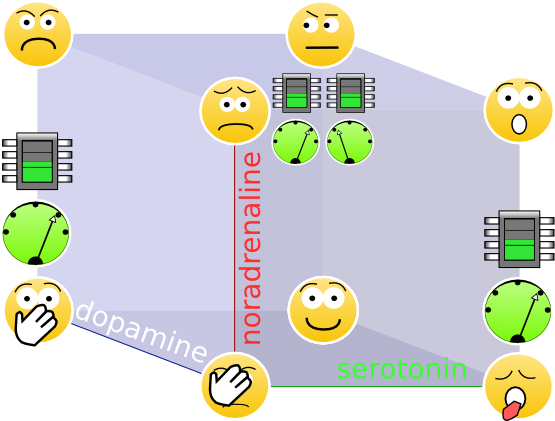
\includegraphics[width=0.8\linewidth]{cube_of_emotional_parameters_machine}
\end{figure}
%------------------------------------------------
\end{columns}
\end{frame}
%------------------------------------------------
\subsection{DA}
%------------------------------------------------

\begin{frame}
\frametitle{Emotional drives: dopamine (DA) pathways}
\begin{figure}
\includegraphics[width=0.8\linewidth]{dopamine_diagram}
\end{figure}
\end{frame}

%------------------------------------------------
%------------------------------------------------

\begin{frame}
\frametitle{DA results: fear-like}
\begin{figure}
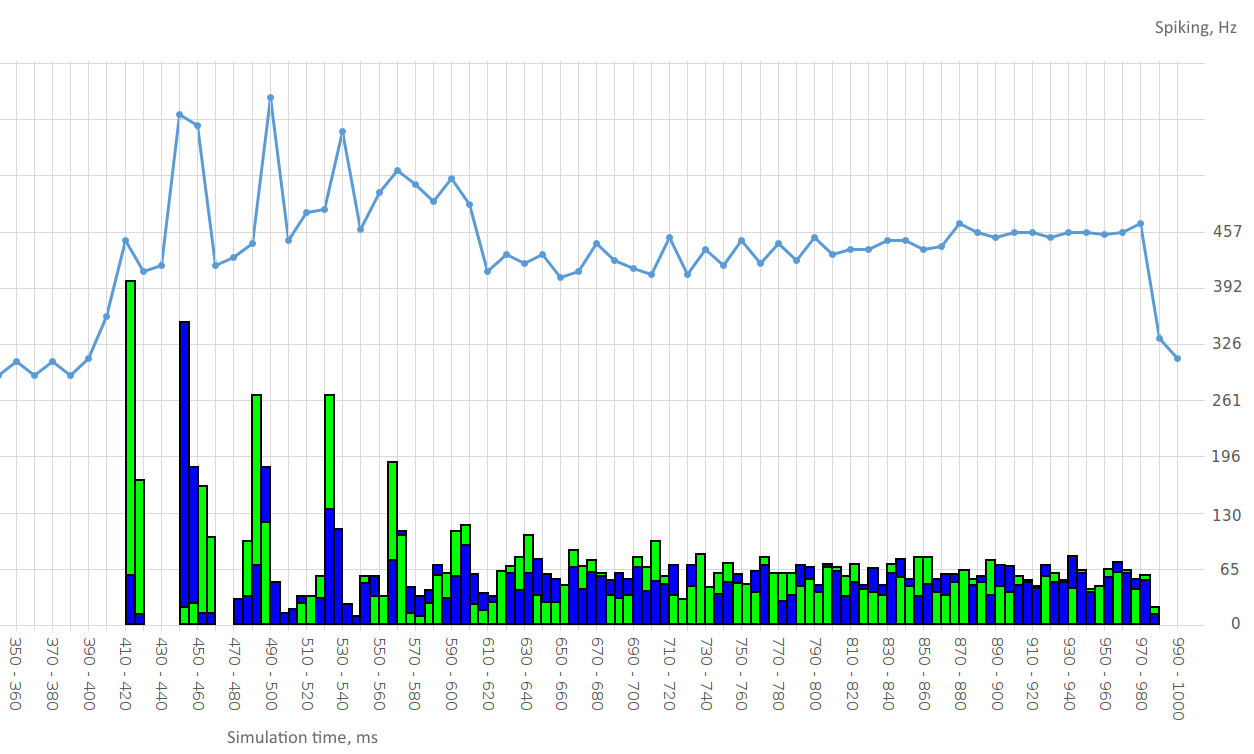
\includegraphics[width=0.6\linewidth]{resultBIG_short}
\end{figure}
400 - 600 ms - simulated brain in placed in the ``fear-like'' state that is indicated with increased level of neuronal activity on motor cortex and thalamus as well as increased computational power consumption.
\end{frame}

%------------------------------------------------
\subsection{5HT}
%------------------------------------------------

\begin{frame}
\frametitle{Emotional drives: serotonin (5HT) pathways}
\begin{figure}
\includegraphics[width=0.7\linewidth]{serotonin_diagram}
\end{figure}
\end{frame}

%------------------------------------------------
%------------------------------------------------

\begin{frame}
\frametitle{5HT results: disgust-like}
\begin{figure}
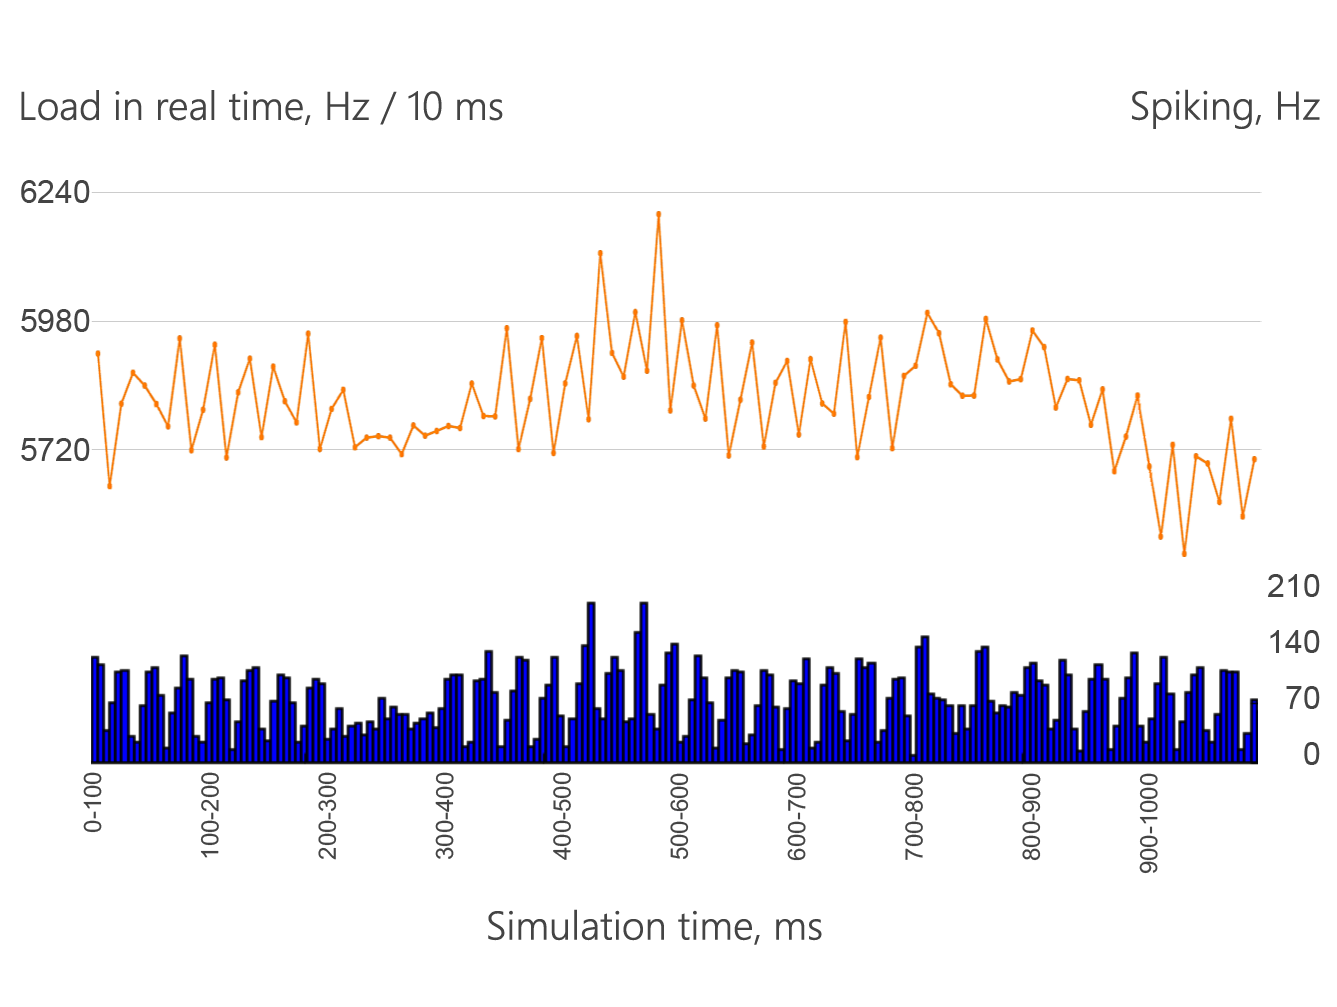
\includegraphics[width=0.6\linewidth]{5ht_results}
\end{figure}
200 - 300 simulated brain in placed in the ``disgust-like'' that is indicated with decreased level of neuronal activity on motor cortex and computational power.
\end{frame}

%------------------------------------------------
\subsection{NA}
%------------------------------------------------

\begin{frame}
\frametitle{Emotional drives: noradrenaline (NA)}
\begin{figure}
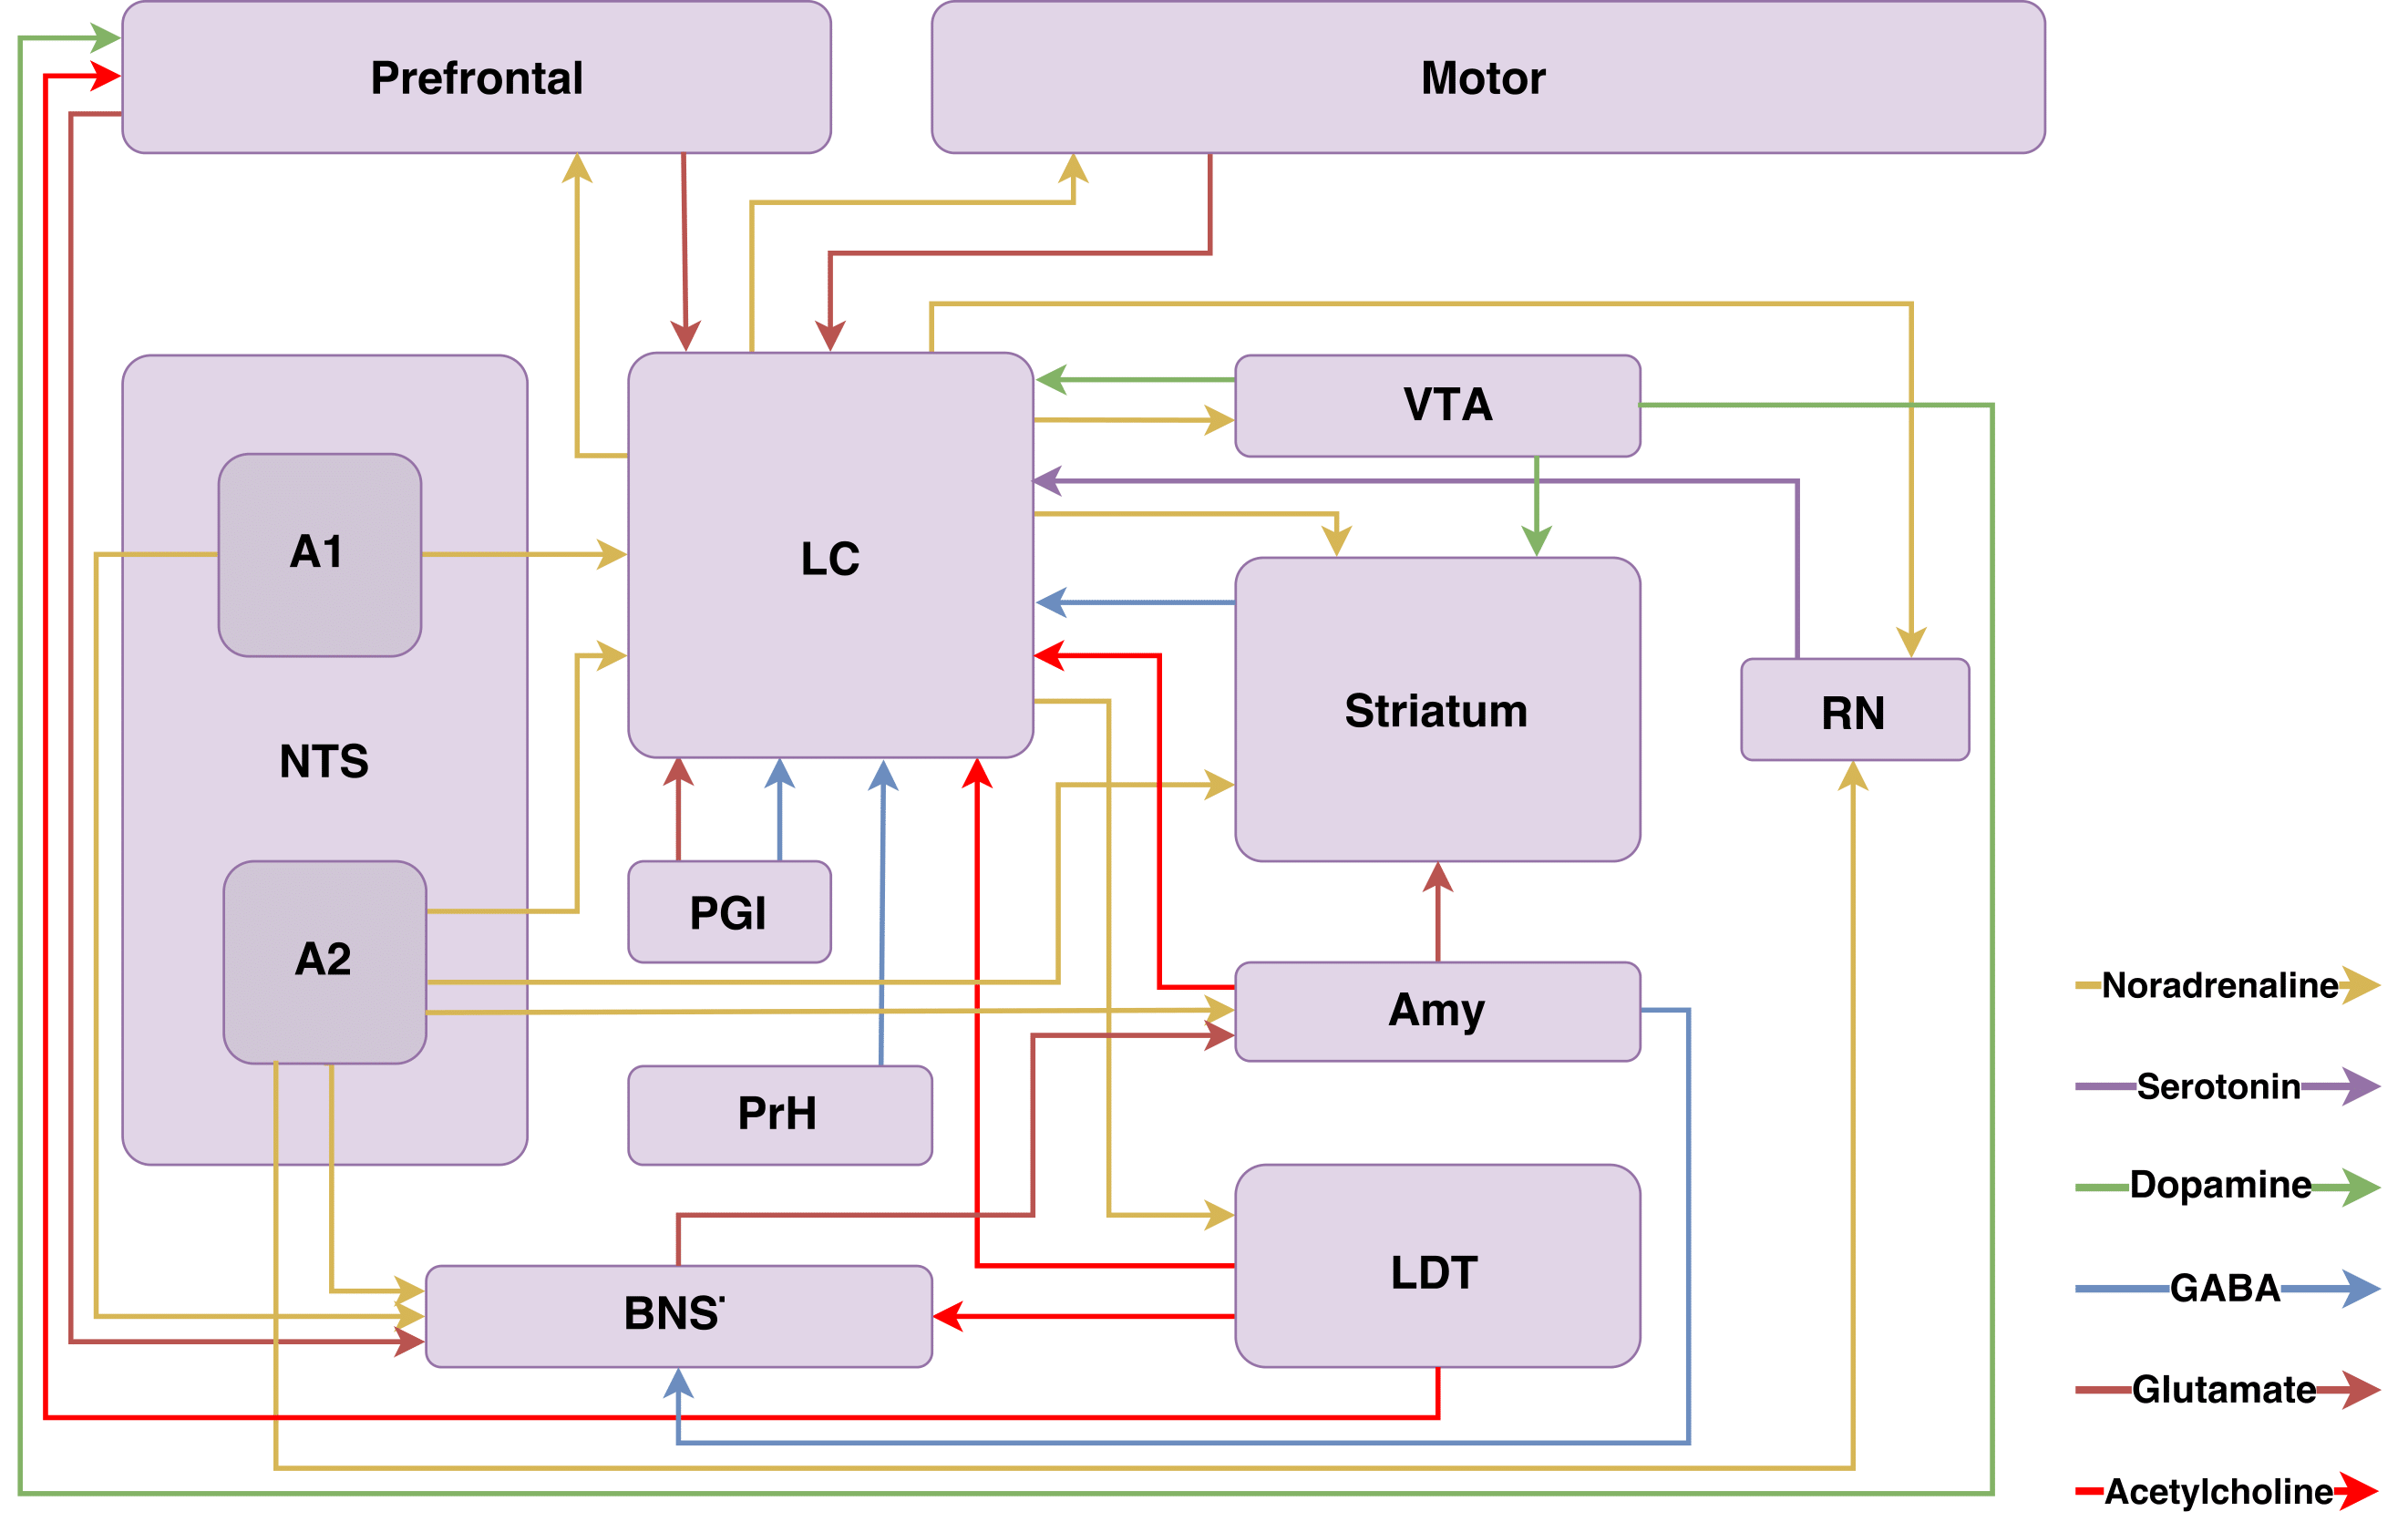
\includegraphics[width=0.7\linewidth]{na_diagram}
\end{figure}
\end{frame}

%------------------------------------------------
\section{Memristive brain}
%------------------------------------------------

\begin{frame}
\frametitle{\#2 Memristive brain}
\begin{figure}
\includegraphics[width=0.8\linewidth]{HL_Emristor}
\end{figure}
\end{frame}

%------------------------------------------------
\section{Integration and Robot dream}
%------------------------------------------------

\begin{frame}
\frametitle{\#3 Integration and Robot dream}
\begin{figure}
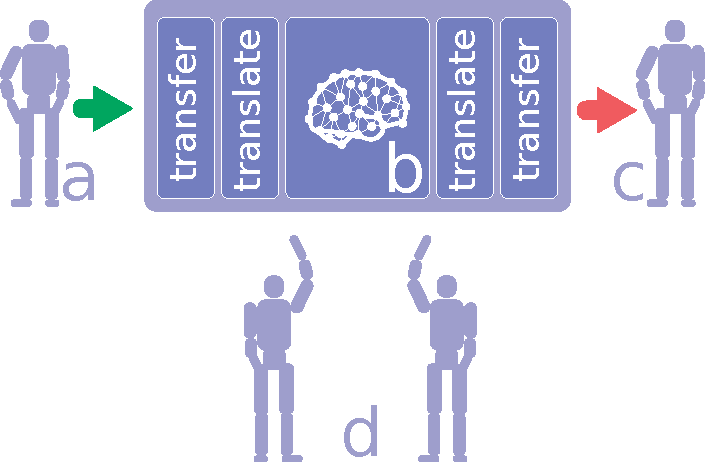
\includegraphics[width=0.8\linewidth]{robot-dream}
\end{figure}
\end{frame}

%------------------------------------------------
\section{Future work}
%------------------------------------------------

\begin{frame}
  \frametitle{Future work}
  
\begin{itemize}
  \item Simple prototype as feasibility study.
  \item \ldots\
  \item Emotional robot with real-time embodiment
  \item Social robot with emotions
  \item Conscious social robot
\end{itemize}

\end{frame}

%------------------------------------------------
%------------------------------------------------

\end{document} 
